\documentclass[12pt]{article}

%%novalidate

\usepackage{tikz}
\usepackage{calc}
\usepackage{booktabs}
%\usepackage{hyperref}
\usepackage[utf8]{inputenc}
\usepackage[T1]{fontenc}
\usepackage{graphicx}
\usepackage{xcolor}
\usepackage{kotex}

%소스코드 추가를 위한 패키지
\usepackage{listings}

\definecolor{codegreen}{rgb}{0,0.6,0}
\definecolor{codegray}{rgb}{0.5,0.5,0.5}
\definecolor{codepurple}{rgb}{0.58,0,0.82}
\definecolor{backcolour}{rgb}{0.95,0.95,0.92}

\lstdefinestyle{mystyle}{
	backgroundcolor=\color{backcolour},   
	commentstyle=\color{codegreen},
	keywordstyle=\color{magenta},
	numberstyle=\tiny\color{codegray},
	stringstyle=\color{codepurple},
	basicstyle=\footnotesize,
	breakatwhitespace=false,         
	breaklines=true,                 
	captionpos=b,                    
	keepspaces=true,                 
	numbers=left,                    
	numbersep=5pt,                  
	showspaces=false,                
	showstringspaces=false,
	showtabs=false,                  
	tabsize=2
}

\lstset{style=mystyle}

% colors
\definecolor{color1}{HTML}{000060}
%\definecolor{color1}{HTML}{8C260F}
\definecolor{color2}{HTML}{333333}


% fonts
\usepackage{fontspec}
\defaultfontfeatures{Mapping=tex-text}
\setmainfont
[BoldFont=HDHarmony_B.ttf,
ItalicFont=Lato-Italic.ttf,
BoldItalicFont=Lato-BoldItalic.ttf]
%{Lato-Regular.ttf}
{HDHarmony.ttf}
\newfontfamily\headingfont[ItalicFont=Lato-BlackItalic.ttf]{HDHarmony_B.ttf}
%%%

\usepackage{geometry}
\geometry{a4paper,
hmargin=20mm,vmargin=20mm,
head=0ex,foot=3ex}

\linespread{1.3}

\usepackage[hang]{caption}
\DeclareCaptionFormat{upper}{#1#2\uppercase{#3}\par}
\captionsetup{labelfont={bf,color=color2},textfont={normalsize,color=color2},format = upper,figurename=FIGURE,tablename=TABLE}

%%% fancy sections
\usepackage{titlesec}
%\titleformat{\chapter}{\headingfont\LARGE\bfseries\scshape\color{color1}}{\thechapter}{1em}{}[\titlerule]
%\titleformat{\section}{\color{color1}\headingfont\Large\bfseries\uppercase}{\thesection}{1em}{}[\titlerule]
%\titleformat{\subsection}{\color{color1}\headingfont\large\bfseries\uppercase}{\thesubsection}{1em}{}
%\titleformat{\subsubsection}{\color{color1}\headingfont\bfseries\uppercase}{\thesubsubsection}{1em}{}
%Title의 재목이 항상 대문자로 표시되기 때문에, \uppercase 문을 삭제함
\titleformat{\section}{\color{color1}\headingfont\Large\bfseries}{\thesection}{1em}{}[\titlerule]
\titleformat{\subsection}{\color{color1}\headingfont\large\bfseries}{\thesubsection}{1em}{}
\titleformat{\subsubsection}{\color{color1}\headingfont\bfseries}{\thesubsubsection}{1em}{}
%%%

% head and foot
\usepackage{fancyhdr}
\pagestyle{fancy}
\lhead{}
\chead{}
\makeatletter
\rhead{\color{color2}\@date}
\makeatother
\newlength{\myheight}
\lfoot{
\settoheight{\myheight}{\thepage}
\raisebox{-2ex-0.5\myheight}{
\includegraphics[height=4ex]{HMC_logo}}
}
\cfoot{\color{color2}ccOS Document}
\rfoot{\color{color2}\thepage}
\renewcommand\headrulewidth{0pt}
\renewcommand\footrulewidth{0pt}

%%% picture on cover page
\usepackage{eso-pic}
\newcommand\BackgroundPic{%
\put(0,0){%
\parbox[b][\paperheight]{\paperwidth}{%
\vfill
\centering
% Cover page의 그림은 일단 삭제
%
\includegraphics[width=\paperwidth,height=\paperheight,%
%keepaspectratio]{cover}%
\vfill
}}}
%%%
% custom titlepage
\makeatletter
\renewcommand{\maketitle}{
\thispagestyle{empty}
\AddToShipoutPicture*{\BackgroundPic}
\ClearShipoutPicture
%
\phantom{a}
\vfill
\phantom{a}\hfill
%    \color{black}\headingfont\LARGE\@title\\[1em]
%    \color{black}\headingfont\Large\@author\\[2em]
\begin{tabular}[c]{@{}p{0.7\textwidth}@{}}
%      \color{white}\headingfont\LARGE\@title\\[1em]
 %     \color{white}\headingfont\Large\@author\\[2em]
     \color{black}\headingfont\LARGE\@title\\[1em]
    \color{black}\headingfont\Large\@author\\[2em]
\end{tabular}
%
\clearpage
}
\makeatother
%%%


%%% fancy boxes
\usepackage{tcolorbox}
\usepackage{wrapfig}
\def\fullboxbegin{
\bigskip
\begin{tcolorbox}[colback=color1,colframe=color1,coltext=white,arc=0mm,boxrule=0pt]
}
\def\fullboxend{\end{tcolorbox}\medskip}
%
\def\leftboxbegin{
\begin{wrapfigure}{l}{0.5\textwidth}
\begin{tcolorbox}[colback=color1,colframe=color1,coltext=white,arc=0mm,boxrule=0pt]
}
\def\leftboxend{
\end{tcolorbox}
\end{wrapfigure}
}
%
\def\rightboxbegin{
\begin{wrapfigure}{r}{0.5\textwidth}
\begin{tcolorbox}[colback=color1,colframe=color1,coltext=white,arc=0mm,boxrule=0pt]
}
\def\rightboxend{
\end{tcolorbox}
\end{wrapfigure}
}
%
\newcounter{frames}
\def\frameboxbegin#1{
\bigskip
\refstepcounter{frames}
\begin{tcolorbox}[colback=white,colframe=color1,arc=0mm,title={\MakeUppercase{\textbf{Frame \arabic{frames}}: #1}}]
}
\def\frameboxend{
\end{tcolorbox}
}

\newcounter{subsubsubsection}[subsubsection]
\def\subsubsubsectionmark#1{}
\def\thesubsubsubsection {\thesubsubsection 
	.\arabic{subsubsubsection}}
\def\subsubsubsection{\@startsection
	{subsubsubsection}{4}{\z@} {-3.25ex plus -1
		ex minus -.2ex}{1.5ex plus .2ex}{\normalsize\bf}}
\def\l@subsubsubsection{\@dottedtocline{4}{4.8em}
	{4.2em}}


%\newcommand{cmd}[args][default]{def}
%%%

\titleformat{\paragraph}[hang]{\normalfont\normalsize\bfseries}{\theparagraph}{1em}{}
\titlespacing*{\paragraph}{0pt}{3.25ex plus 1ex minus .2ex}{0.5em}

\titleformat{\subparagraph}
{\normalfont\normalsize\bfseries}{\thesubparagraph}{1em}{}
\titlespacing*{\subparagraph}{\parindent}{3.25ex plus 1ex minus .2ex}{.75ex plus .1ex}

\usepackage{indentfirst}
\setlength{\parindent}{0.5cm}% too much in my eyes delete this
% line and use the default ...


%%%%%%%%%%%%%%%%%%%%%%%%
% Section 넘버링 depth 설정
\setcounter{secnumdepth}{5}
\setcounter{tocdepth}5


%%%%%%%%%%%%%%%
% Title Page
\title{Study Note for Deep Learning}
\author{Se Won Kim}
\date{\today}
%%%%%%%%%%%%%%%

\begin{document}
	\maketitle
	
	\tableofcontents
	
	%%%%%%%%%%%%%%%%%%%%%%%%%%%%%%%%%%%%%%%%%%%%%%%%%%
	% 본문의 시작 
	%%%%%%%%%%%%%%%%%%%%%%%%%%%%%%%%%%%%%%%%%%%%%%%%%%

		\clearpage
	\section{서론}
	
	본 문서는 최근 다양한 분야에서 관심을 받고 자주 언급되는 deep learning에 대해 동민이와 나만 이해하기 위한 문서이다. 도대체 이놈의 Deep learning이라는 것이 얼마나 대단한 것이길레 앞으로의 세상을 변화한다고 떠들어 대고, 툭하면 4차 산업이니 머니 해서 너님들의 직업이 앞으로 사질거다 말거다 협박하는 시대의 흐름에 좀더 AI라는 것에 잘 알아보고자 문서 작성을 시작하였다. 사실은 동민이가 나의 AI에 대한 호기심을 크게 자극했기 때문에 시작한 것이다. 
	
	이 글을 쓰기 시작한 시점에 나는 Deep learning에 대한 기초적인 지식이 없는 상황이고 심지어 내용에 소개되는 편미분에 대한 정의까지 까먹고 있을 정도로 deep learning을 이해할 준비가 안된 상태이기도 하다. 이러한 이유로 내가 서술한 내용 중에서 틀린 내용이 분명 존재 할 것이므로 양해를 부탁한다.
	
	\subsection{어디서 부터 시작할 것인가?}
	Deep learning에 대해 잘 알지 못하는데 deep learning을 공부하기 위하면 어떻게 하는 것이 좋을까? Deep learning을 알기 위해서 출발점은 무엇일까? 학부때 배운 인공지능 책 부터 보는 것이 좋을까? 적어도 학부 전공 서적부터 보는 것은 좋은 생각은 아닌 것 같다는 생각이 들었다. 
	
	\begin{figure}[!h] %Deep Learning책 표지
	\centering
	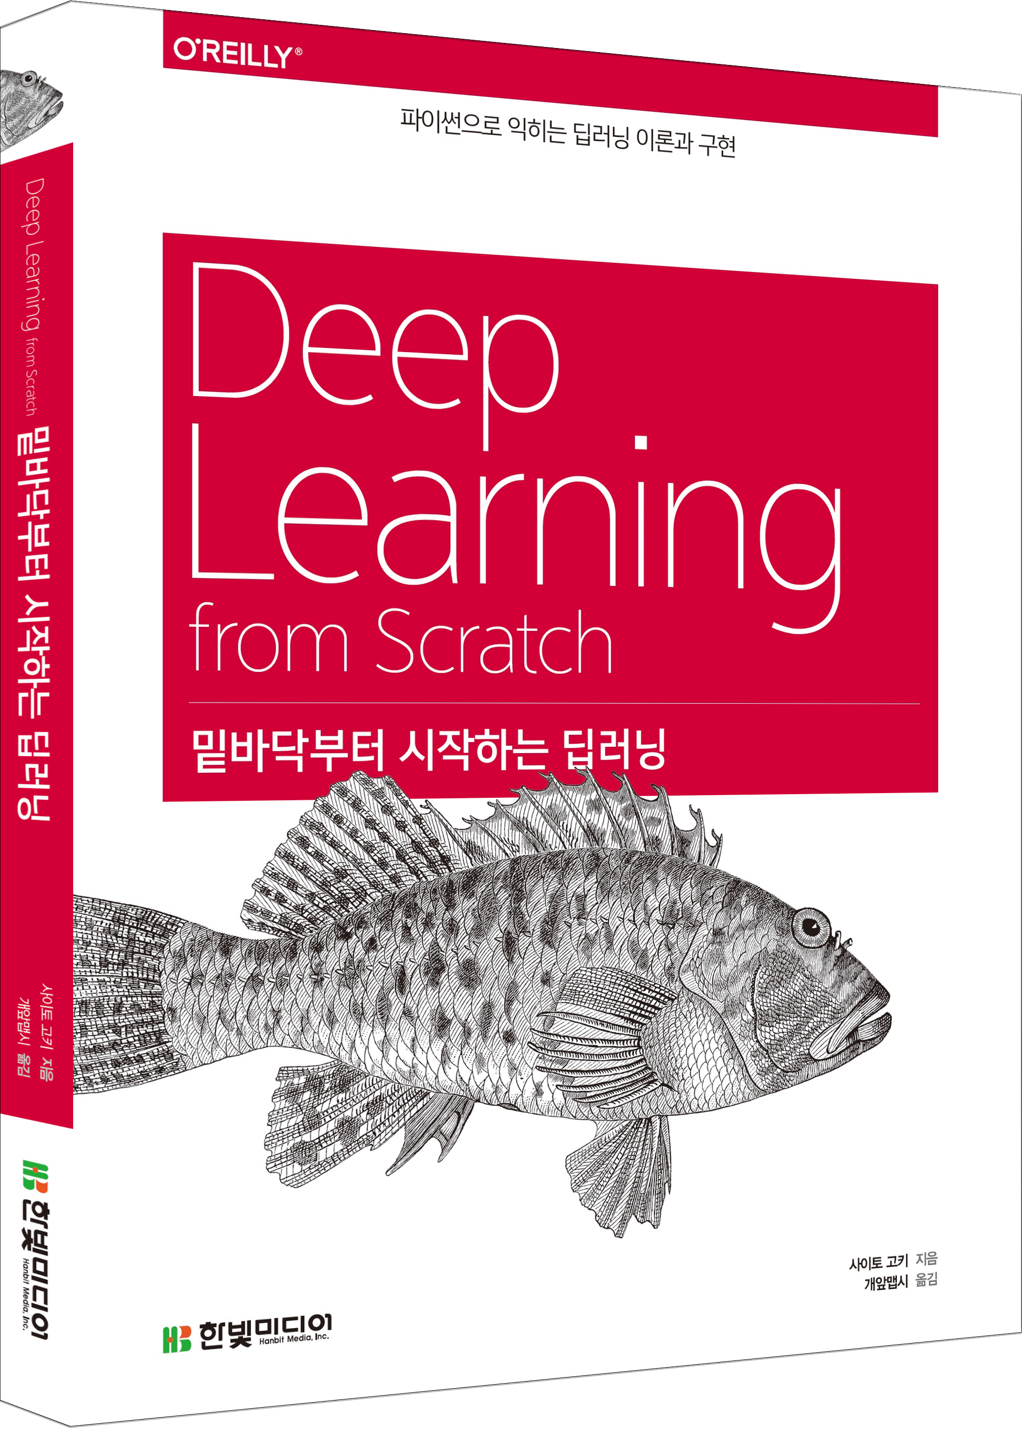
\includegraphics[width=0.5\textwidth]{fig/cover_image.jpg}
	\caption{Deep Learning의 시작으로 삼은 "Deep Learning from Scratch"}
	\label{fig:DL_book_cover}
	\end{figure}
	
	그림 \ref{fig:DL_book_cover}은 내가 deep learning을 배우기 위한 시작점으로 삼은 책이다. 이 책은 우연히 서점에서 발견한 책이고 두 가지가 문구가 나로 하여금 이 책을 선택하게 했다. 첫번째 문구는 제목에서 보인 ``from scratch'' 이다. 밑바닥 부터 시작한다는 뜻이니까, deep learning에 대해 모르는 사람들에게도 아주 기초적인 개념부터 하나씩 차근차근 설명해 주겠다는 친절한 문구이다. 그리고 실제로 내용또한 deep learning을 모르더라도 차근차근 이해할 수 있는 내용들로 구성되었다.
	
	두번째 문구는 표지 상단에 있는 ``파이썬으로 익히는''이라는 문구이다. 파이썬 덕후인 나로서 매우 반가운 문구가 아닐수 없다. 뿐만 아니라, 내용을 얼핏 보니 책의 각 장에서 설명한 개념을 친절하게도 파이썬 코드로 하나하나 설명해 줬다. 게다가 타이핑하기 귀찮으면 Github에서 clone해서 쓰란다.
	
	이러한 두 문구로 이 책을 선택했고, 읽고 내용에 감동하여 지금 이렇게 잉여력을 발휘하여 글을 쓰고 있다.
	
	\subsection{책의 간략한 구성}
	책의 1장은 파이썬의 간단한 문법과 deep learning구현을 위한 라이브러리(numpy)를 소개한다. 파이썬을 안다면 넘어가도 좋다. 혹시 안다고 해도 numpy 설명 부분은 한번쯤은 봐두자.
	
	2장은 퍼셉트론에 대해 설명한다.  퍼셉트론은 신경망에 기원이 되는 알고리즘이라서 소개 한다고 한다. 어떤가 벌써 부터 ``from scratch''라는 공약을 지키는 모습을 보여준다.
	
	3장은 이제 퍼셉트론에 활성화 함수라는 것을 덫붙이고 퍼셉트론을 여러개 붙이는 그럴싸한 신경망이란 것을 소개한다. 2장의 내용을 확장한 것이라 보면 된다. 퍼셉트론이라는 deep leaning이라는 연산의 기본 단위를 확장해서 퍼셉트론이 모이면 어떤 큰 일을 할 수 있는지를 보여준다.
	
	4장은 신경망이 어떻게 스스로 자기 자신을 개선하는지를 보여준다. 이때 손실함수, 경사 하강법이 등장한다. 손실 함수는 퍼셉트론의 각 노드에 대한 가중치로 인한 결과에 대한 정량적인 평가 방법이다. 마치 노드의 가중치를 얼마얼마 주고 답을 알고 있는 데이터로 학습 시켰을때 ``음 그렇게 가중치 주면 70점짜리 결과를 보인다.''라는 식의 결과를 산출하는 방법이다. 
	
	이렇게 손실 함수로 우리가 퍼셉트론 가중치의 학습 결과를 평가 할 수 있다면 평가 점수가 가장 높게 받을 수 있는 가중치 값을 찾으면 훌륭한 신경망을 만들 수 있게 된다. 최적의 가중치 값을 찾는 방법중 하나가 경사 하강법이다. 손실함수는 어찌 되었건 간에 퍼셉트론의 가중치 값에 대한 평가 결과를 계산하고 그것을 시각화 해보면 가중치를 각각의 차원 축으로 하는 임임의 차원 공간에 물체로 그려질 것이다. 이때 대입한 각 가중치에 대한 미분값을 통해 현재 가중치 값에서 어느 방향으로 진해하면 손실함수의 평가 결과를 좋게 받을 수 있을지를 알 수 있게 된다.
	
	정리 하자면, 4장은 신경망을 구성하는 퍼셉트론의 가중치와 그 가중치를 평가하고 개선하는 알고리즘을 소개 한다.
	
	5장은 오차역전파법이라는 괴랄한 이름의 알고리즘을 소개한다. 쉽게 말하면 4장에서 소개한 편미분을 이용한 경사 하강법이 사실은 엄청난 계산량을 요구하고 이를 개선한 방법이다. 5장은 매우 중요 하지만 전체적인 큰 흐름을 이해하고 싶다면 넘어가도 좋다.
	
	6장또한 부가적인 내용이긴 하지만 알아두면 도움이 될 것 같다. 하지만 시간이 없다면 스킵~~. 5장은 4장에서 소개한 편미분을 계산량을 획기적으로 줄이는 방법을 제시했다면 6장은 4장에서 소개한 가중치를 개선하는 전략은 경사 하강법의 보완 버전들을 소개한다. 알아두면 좋지만, 전체 흐름의 이해가 우선이라면 스킵해도 좋다.
	
	7장은 CNN이라는 합성곱 신경망을 소개한다. 요건 좀 중요한데, 앞서 신경망은 인풋 데이터를 1차원 배열로 놓고 풀지만, CNN부터는 데이터를 있는 그대로 처리하는데 초점을 맞춘다. 간단히 예를 들자면, 이미지 처리를 할경우 신경망은 2차원 이미지 데이터를 1차원 배열로 변경하여 문제를 푼다. 반면 CNN은 이미지 데이터를 있는 그대로 2차원 배열로 받아서 인식을 한다. 이를 위해 "합성곱(혹은 필터 연산이로고도 한다.)", "패딩", "스트라이드", "풀링"을 설명한다. 이 부분을 읽을때 꼭 이해해야할 중요한 컨셉이다.
	
	8장은 마지막 장으로 CNN 진화 버전으로 딥러닝이라 불리우는 다양한 기술에 대해 설명한다.
	
	정리 하자면,7장의 CNN을 설명하기 위해 2,3,4장에서 퍼셉트론, 신경망, 신경망 학습을 설명한다. CNN을 설명했으니 CNN을 이용해서 현재의 deep learning 최신 기술을 8장에서 설명할 수 있던 것이다.
	
	
		\clearpage
	\section{퍼셉트론}
	
	\subsection{키워드}
	이번 장에서는 다음 키워드를 이해했다면, 그대는 성공~
	\begin{itemize}
		\item 노드(Node)
		\item 가중치(Weight)
		\item 편향, 임계값(Bias, $\theta$)
	\end{itemize}
	
	\subsection{정의}
	퍼셉트론은 다수의 입력을 받아 ``자체 연산''을 통해 출력 신호를 만들어 낸다. 이때 출력 신호는 0 또는 1이다. 입력 신호는 임의의 수만큼 받을 수 있다. 퍼셉트론은 각 입력 신호에 가중치를 곱한 값들을 합한다. 그리고 가중치를 곱한 값의 합이 임계값 보다 크면 1 임계값보다 작으면 0을 출력 신호로 만든다. 여기에서 입력 신호의 가중치를 곱하고 그들을 더하여 임계값과 비교하는 것을 퍼셉트론의 ``자체 연산''이다.
	


	편향(bias)는 뉴런이 얼마나 쉽게 활성화 되는지를 제어한다.
	가중치는 각 신호의 영향력을 의미한다.
	
	
	Perceptron은 복잡한 함수도 표현이 가능하다. 심지어 다층 퍼셉트론은 컴퓨터도 표현 가능하다.
	하지만, 퍼셉트론의 가중치를 설정하는 것은 여전히 사람에 의해서만 가능하다.
	
	신경망은 데이터로 부터 퍼셉트론의 가중치 설정을 자동으로 한다.
	

	\clearpage
	\section{신경망}
	
	\begin{figure}[!h] %신경망 예시 그림
		\centering
		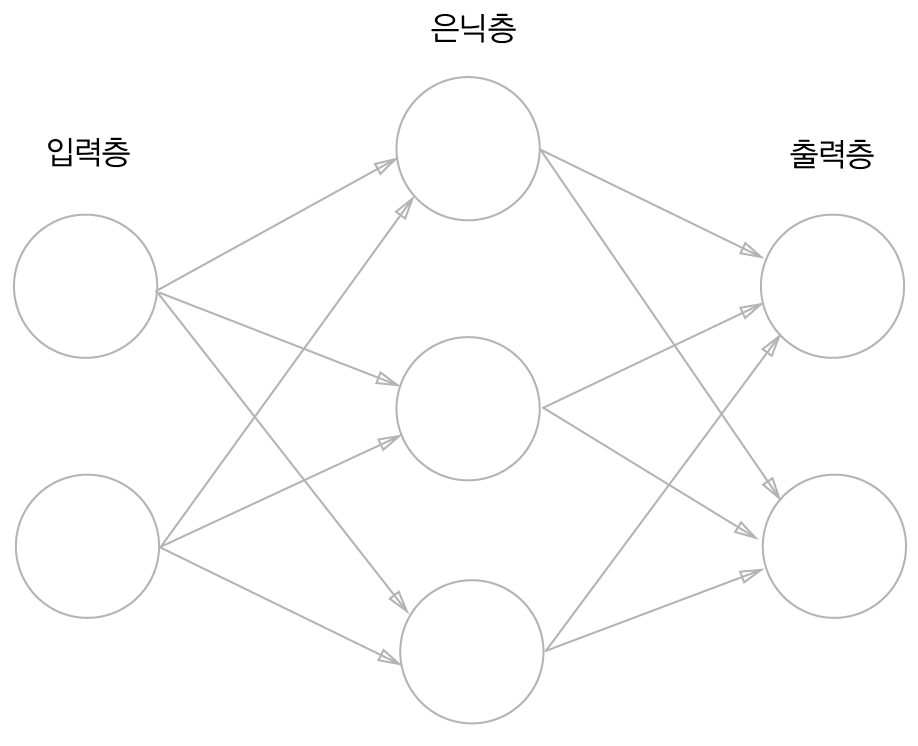
\includegraphics[width=0.8\textwidth]{fig/fig-3-1.png}
		\caption{신경망의 예}
	\end{figure}
	
	
	입력층, 은닉층, 출력층 으로 구성
	활성화 함수 - 입력 신호의 총합을 출력 신호로 변환
	
	활성화 함수를 계단 함수에서 다른 함수로 변경하는 것이 신경망의 세계로 나아가는 열쇠이다.
	
	% $f(x)=\frac{1}{1+e^{-x}}$
	\[ f(x)=\frac{1}{1+\exp^(-x)}	\]
	
	신경망의 활성화 함수는 비선형 함수를 사용해야 한다. 여기서 비선형이란 하나의 직선으로 표현할 수 없는 함수를 의미한다.
	비선형 함수를 사용하는 이유는 선형 함수를 사용할 경우 신경망 층을 깊게 하면 의미가 사라지기 때문이다.
	
	신경망은 분류와 회귀에 이용할 수 있다. 이는 출력층의 활성화 함수의 선택을 결정 짓는 요인이 된다. 회귀에는 항등함수를 사용하고 분류에는 소프트맥스함수를 사용한다.
	
	\subsection{소프트맥스 함수의 특징}
	소프트맥스 함수의 출력은 0과 1.0사이의 실수이며, 함수 출력 총합은 1이다.
	이러한 성질을 이용하면 소프트맥스 함수의 출력을 확률로 생각할 수 있다.
	\[ f(v) = \frac{\exp(a_{k})} {\sum_{i=1}^{n}  {\exp(a_{i})}} \]
	
	소프트맥스 함수는 단조 증가 함수이기 때문에 소프트맥스 함수를 활성함수로 적용해도 각 원소의 대소 관계는 변화가 없다. 따라서, 신경망을 이용하여 분류를 할때 출력층의 소프트맥스 함수를 생략할 수 있다.
	
	\subsection{궁금한점}
	하지만, 분류에 소프트맥스 함수를 생략 할 수 있다면 결국 항등 함수와 무엇이 다른가?
	\clearpage
	
\section{신경망 학습}
학습이한 데이터로 부터 가중치 매개 변수의 최적값을 자동으로 획득한다.
그렇다면 어떻게 매개 변수가 최적값인지를 판단할 수 있을까?
즉, 매개 변수에 대한 평가 방법이 필요하며 이러한 역할은 손실 함수가 수행한다.
손실 함수가 매개 변수 성능에 대한 결과를 정량적인 수치로 나타낸다면, 
신경망의 학습 목표는 손실 함수의 값을 작게 만드는 매개 변수를 찾는 것이다.

어떻게 하면 손실함수의 값을 작게 만들 수 있을까?
이는 손실 함수와 매개 변수와의 관계를 다시 생각해 보게 한다.
매개 변수가 손실 함수에 미치는 영향을 분석하여 각 매개 변수가 음(-)이나 양(+)의 방향과 그 정도를 통해
손실 함수를 가능한한 최소화하는 값을 찾을 수 있고 이러한 방법을 경사법이라 한다.


딥러닝은 종단간 기계학습(end-to-end machine learning)이라고도 한다. 데이터(입력)에서 목표한 결과(출력)을 사람의 개입없이 얻는다는 의미.

\subsection{손실함수}

손실함수는 평균 제곱 오차(mean squared error, MSE)와 교차 엔트로피 오차(cross entropy error, CEE) 둘이 자주 사용된다.
\subsubsection{평균 제곱 오차}
평균 제곱 오차의 식은 다음과 같다.
\[ E = \frac{1}{2} \sum_{k}(y_{k} - t_{k})^2  \]

이때 궁금한 점은 평균임에도 불구하고 왜 n이 아닌 2로 나누는 것인가? 이는 y값과 t값이 갖는 범위를 생각해 보면 이해할 수 있다. 먼저 y는 소프트맥스함수 값이므로 $y_{k}$ 총 합은 항상 1이다.
$t_{k}$는 원-핫 인코딩으로 표기 했기 때문에 정답에 해당하는 값만 1이고 나머지는 0이다. 따라서 $t_{k}$의 총합 또한 항상 1이다. 따라서 이들의 평균을 구하기 위해서는 N이 아닌 2로 나누어야 한다.

평균 제곱 오차의 값이 작을 수록 정답에 가깝고 값이 클 수록 정답이 아님을 의미한다.
	\subsubsection{교차 엔트로피}
	교차 엔트로피는 

\subsection{ 편미분}
\begin{lstlisting}[language=Python, caption={Python으로 구현한 편미분 함수},label=gradient-function]
def numerical_gradient(f, x):
	h = 1e-4
	grad = np.zeros_like(x)

	for idx in range(x.size):
		tmp_val = x[idx]
		x[idx] = tmp_val + h
		fxh1 = f(x)

		x[idx] = tmp_val - h
		fxh2 = f(x)

		grad[idx] = (fxh1 - fxh2) / (2*h)
		x[idx] = tmp_val

	return grad
\end{lstlisting}

Listing \ref{gradient-function}은 편미분을 구하는 python함수이다. Line1의 함수의 선언에서와 같이 편미분을 구하는 numerical\_gradient함수는 인자로 편미분을 구하고자 하는 함수 f와 그때의 좌표를 np.array형인 x로 받는다.

\clearpage
\section{오차역전파법}

\clearpage
\section{학습관련기술들}

\clearpage
\section{합성곱 신경망}

\clearpage
\section{딥러닝}


\end{document}          
